\section{Results and Evaluation}

One of the objectives of this project is to react to events, which is why recent information is crucial to all of the models developed. Consider the two contrasting examples: 1) if there has been a collision on the road, all buses that use this route will be delayed compared to 2) if a bus driver is in an argument with one of the passengers getting on the bus, then only that particular bus would be delayed, not any of the other buses on the route. In the first case, the desired outcome is indeed to react to this increase in journey time and provide predictions with longer than usual journey times. However, in the second case, the `delay' is localised to that particular bus and so predictions should not provide predictions with longer than usual journey times. Therefore, it is possible to overreact to situations and adjust the prediction when there is not an actual cause for the model to do so. \\

In the context of bus journey times, the mean absolute error (MAE) and the root mean squared error (RMSE) mean different things and provide different insights. The MAE results describe how many seconds off the actual journey time a model consistently predicts. For example, a MAE of 100 seconds implies that the model consistently predicts a journey time of 100 seconds more or less than the actual journey time (although it does not provide insight into whether the model over or under predicts). On the other hand, since the errors are squared before they are averaged, the RMSE gives a relatively high weight to large errors. This penalization of large errors could be appropriate if for example, a prediction that is four minutes off is more than twice as bad as a prediction that is two minutes off. This brings to question, what counts as a `good' bus journey prediction? \\ 

So, is a model that predicts journeys that are consistently 3 minutes off better than a model that predicts journeys that are 1 minute off occasionally and 5 minutes off occasionally? In the long run, waiting an extra minute or two doesn't make much of a difference. However, waiting upwards of 5 minutes is significant. This suggests that the RMSE results are more important than the MAE results. On the other hand, if waiting 5 extra minutes is no more than twice as bad as waiting around 2 extra minutes, then the MAE is actually more appropriate. Therefore since this is a fairly subjective issue, for this project, both the MAE and RMSE will be presented. 

\subsection{Historical Model}

First consider the results for journeys between stops that are five apart. \\

Figure \ref{fig:historical-past2hours} shows the predicted journey time versus the actual journey time versus TfL's own predicted journey time. This figure is for buses on route 52 for journeys between Chesterton Road to Notting Hill Gate Station, where the predictions have been found using the historical model that looks back at buses in the past two hours. 

\begin{figure}[H]
\begin{center}
    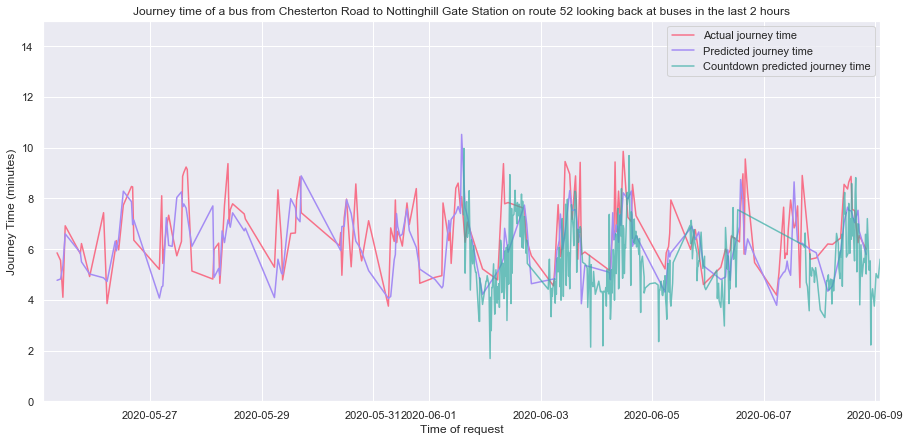
\includegraphics[keepaspectratio, width=15cm]{Images/historical-past2hours.png}
    \caption{Historical Model looking at buses from past two hours}
    \label{fig:historical-past2hours}
\end{center}
\end{figure}

Graphs such as in Figure \ref{fig:historical-past2hours} were also produced for predictions that were found using the historical models that looked back at the past 15 minutes, 30 minutes and 60 minutes. The MAE and RMSE were calculated for all four models that look back X amount of time. The results can be seen in Figure \ref{fig:historical-lookingbacktime}. 

\begin{figure}[H]
\begin{center}
    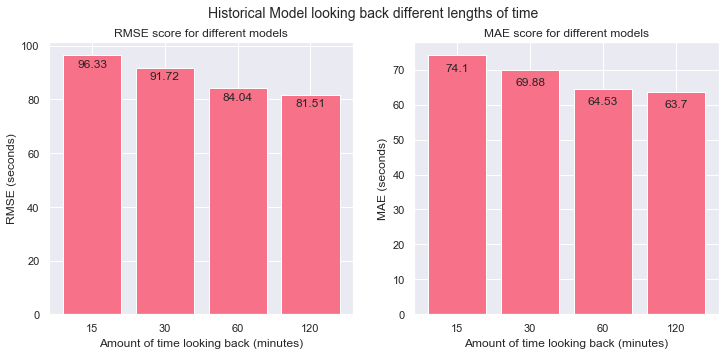
\includegraphics[keepaspectratio, width=15cm]{Images/historical-amountoftime-gap5.png}
    \caption{Historical Model looking back at x amount of time}
    \label{fig:historical-lookingbacktime}
\end{center}
\end{figure}

Consider the model that looks back at journeys from the past 120 minutes. Figure \ref{fig:historical-lookingbacktime} indicates that based on the MAE, the predictions are on average about a minute higher or lower than the actual journey time. This is an excellent result, however, bear in mind that this is only for stops that are five apart. It will be shown later that when these models are applied to stops that are further apart, the MAE and RMSE grow. Since the RMSE is only about 20 seconds more than the MAE, this suggests that either predictions that are significantly off don't occur very often or predictions are generally close to 1 minute off. \\

Intuitively, it makes sense that the model that looks back at the last 15 minutes performs the worst out of the four sub-models presented above. This is because looking at only the past 15 minutes means the probability of overreacting to an event is much higher. In particular, Figure \ref{fig:historical-past2hours} demonstrates that the actual journey time ranges between 4 minutes to 10 minutes and so when the model looks back at the last 15 minutes, it will be looking at most at the last three buses. In the worst case, it would only look back at the last bus. This means that if there is something that causes only that particular bus to delay, the model will not realise that this is an anomalous journey time and so will predict a longer journey time when it should not have. \\

Figure \ref{fig:historical-past2buses} shows the predicted journey time versus the actual journey time versus TfL's own predicted journey time. This figure is also for buses on route 52 for journeys between Chesterton Road to Notting Hill Gate Station. However, here the predictions have been found using the historical model that looks back at the last two buses to complete the journey.

\begin{figure}[H]
\begin{center}
    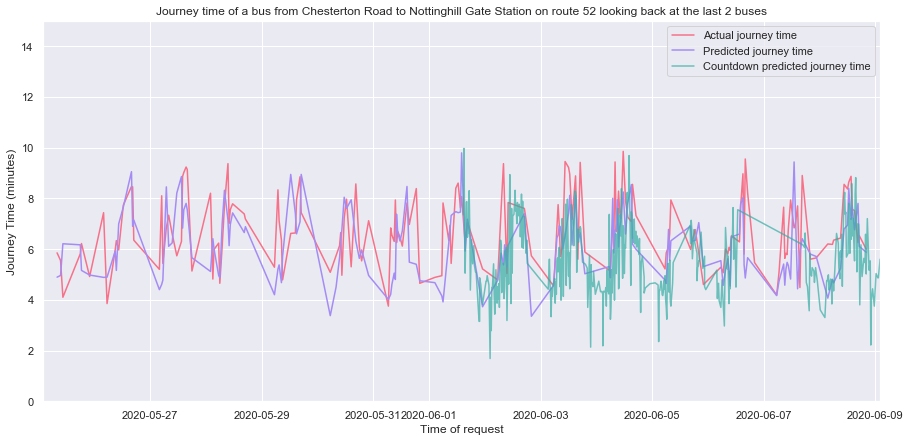
\includegraphics[keepaspectratio, width=15cm]{Images/historical-past2buses.png}
    \caption{Historical Model looking at past two buses}
    \label{fig:historical-past2buses}
\end{center}
\end{figure}

Graphs such as in Figure \ref{fig:historical-past2buses} were also produced for predictions that were found using the historical models that looked back at the past 5 buses, 10 buses and 15 buses. The MAE and RMSE were calculated and can be seen in Figure \ref{fig:historical-lookingbackbuses}.

\begin{figure}[H]
\begin{center}
    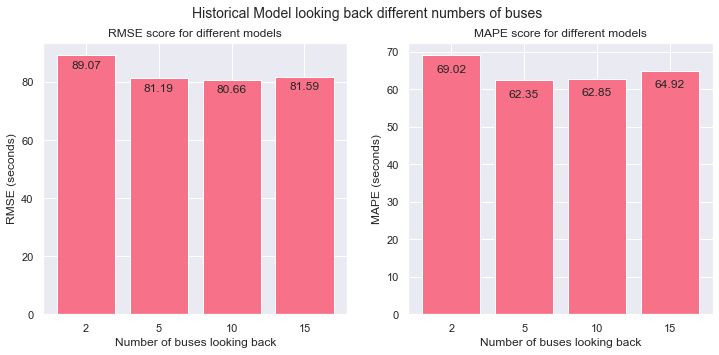
\includegraphics[keepaspectratio, width=15cm]{Images/historical-numberofbuses-gap5.png}
    \caption{Historical Model looking back at x number of buses}
    \label{fig:historical-lookingbackbuses}
\end{center}
\end{figure}

Consider the model that looks back at the last five buses. Based on the MAE, Figure \ref{fig:historical-lookingbackbuses} implies that predictions are on average about a minute more or less than the actual journey time. However, as before, these are results for bus stops that are five apart and so should not be treated as conclusive results. \\

In a similar argument to earlier, it makes sense for the model that looks back at the last two buses to perform the worst out of the four sub-models presented above. This is because of its high probability of overreacting to events. On the other hand, it also makes sense that the model that looks back at the last 15 buses doesn't perform as well as the one that looks back at the last 5 or 10 buses. This is because this model is more likely to take journey times that are no longer relevant into account. For example, consider the following case: a bus is not a 24 hour bus route - its last bus is at 00:30 and its first bus is at 05:25. If a prediction is requested at 05:40, the last 15 buses will include bus journeys made around midnight or before. As mentioned in Section \ref{section:data-exploration}, at different times of day the journey times are not the same. Therefore, the prediction could be less than it should be. Furthermore, if there was some disruption that caused the bus journeys around midnight to be significantly longer or shorter, this too could adversely affect the prediction. However, since its performance is not actually significantly worse than the model that looks back at the last 5 or 10 buses, this could be put down to the weights that were chosen that ensured that bus journeys long before the request time do not have as much impact on the prediction. \\

Figure \ref{fig:historical-gap5-all-compare} shows all eight sub-models' MAE and RMSE for stops that are five apart compared against each other. According to the RMSE the best two models are 1) looking back 10 buses 2) looking back 5 buses. According to the MAE the best two models are 1) looking back 5 buses 2) looking back 10 buses. Overall, this means that the top two sub-models, found by averaging the MAE and RMSE are 1) looking back 10 buses 2) looking back 5 buses. The third and fourth best sub-models overall are 3) looking back 2 hours 4) looking back 15 buses. 

\begin{figure}[H]
\begin{center}
    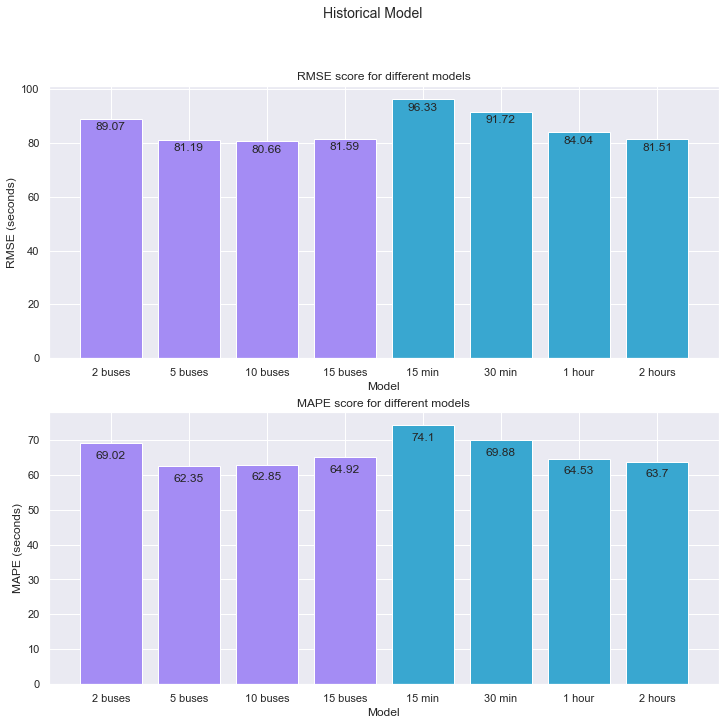
\includegraphics[keepaspectratio, width=15cm]{Images/historical-all-compare-gap5.png}
    \caption{Historical Model}
    \label{fig:historical-gap5-all-compare}
\end{center}
\end{figure}

Figure \ref{fig:historical-gap5-all-compare} shows that the models that look back a certain amount of time have a larger range than the models that look back a certain amount of time. This suggests that the models that look back a certain amount of time are more likely to produce predictions that are further away from the actual value. Therefore, it can be concluded that looking back a specified number of buses is more likely to produce better results than looking back a specified amount of time. The ranges are as follows:

\begin{itemize}
    \item Historical model looking back different amounts of time: RMSE range = 14.82 seconds, MAE range = 10.4 seconds.
    \item Historical model looking back different numbers of buses: RMSE range = 8.41 seconds, MAE range = 6.67 seconds.
\end{itemize}

The best two models were applied to pairs of stops that are larger than five apart. The results for the model that looks back 10 stops are seen in Figure \ref{fig:historical-allgals-lookback10} and the results for the model that looks back 5 stops are seen in Figure \ref{fig:historical-allgaps-lookback5}. 

\begin{figure}[H]
\begin{center}
    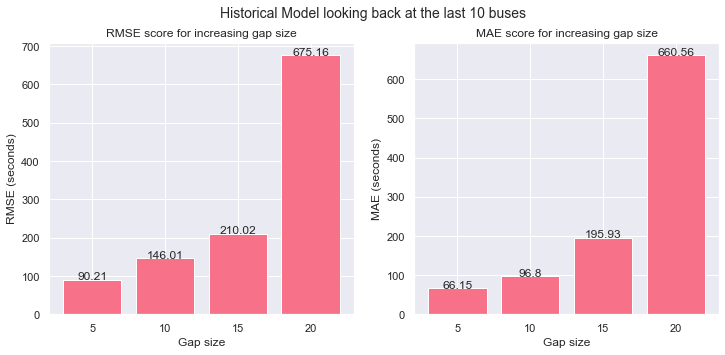
\includegraphics[keepaspectratio, width=15cm]{Images/historical-lookingback10-varyinggaps.png}
    \caption{Looking back at the last 10 journeys}
    \label{fig:historical-allgals-lookback10}
\end{center}
\end{figure}

\begin{figure}[H]
\begin{center}
    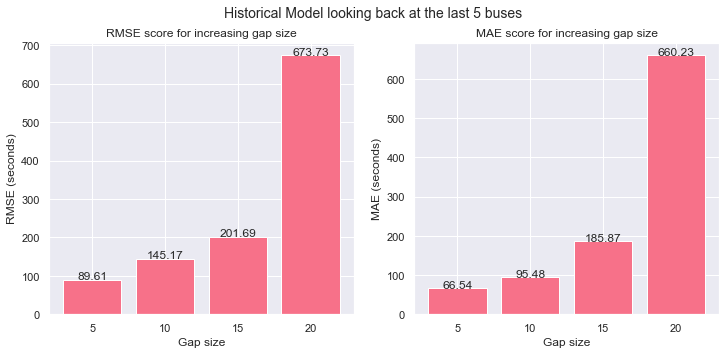
\includegraphics[keepaspectratio, width=15cm]{Images/historical-lookingback5-varyinggaps.png}
    \caption{Looking back at the last 5 journeys}
    \label{fig:historical-allgaps-lookback5}
\end{center}
\end{figure}

It can be seen that for both models, as the distance between the stops grow, so too does the RMSE and MAE. This makes sense because as the stops grow further apart, the standard deviation and variance of the actual journey times also increase. This means that there is a lot more fluctuation in the training times given to the models to calculate a weighted average out of. It can be seen that up to fifteen stops apart, the performance can still be deemed as good, however, it is at gaps of around twenty that the performance drops significantly.  \\

Taking the average of the MAE and RMSE for the different gap sizes for both models gives the following results: 

\begin{itemize}
    \item Historical model looking back at the last 5 buses: RMSE = 277.55 (5sf), MAE = 252.03 (5sf)
    \item Historical model looking back at the last 10 buses: RMSE = 280.35 (5sf), MAE = 254.86 (5sf)
\end{itemize}

It can be seen that the two models have very similar results when looking at their performance across all gap sizes. This suggests that overall, looking back at the last five or ten buses does not make much of a difference in predicting journey times. 

\subsection{Regression + Interpolation Model}

Part 1 of the regression + interpolation model calculates the `global' prediction. The regression model was evaluated on requests made from 20/04/2020 01:00:00 to 08/06/2020 23:59:59 at thirty minute intervals for a number of different pairs of stops of varying routes and gap sizes. The root mean squared error (RMSE), R2-score and mean absolute error (MAE) were then calculated and the results are shown below:

\begin{itemize}
    \item RMSE: 343.09 seconds (5sf)
    \item R2-score: 0.86865 (5sf)
    \item MAE: 224.58 seconds (5sf)
\end{itemize}

Since an R2-score of 1 means a perfect prediction and the R2-score is bounded between 0 and 1, a score of 0.85749 indicates that the model gives a fairly good prediction of the journey time. However, the MAE and RMSE score indicate that the predictions can be around 4 and 6 minutes off respectively, which doesn't seem too great. This supports the hypothesis that recent data, i.e. the `local' conditions, need to also be taken into account as looking at these `global' factors alone does not provide an accurate enough prediction. However, it should be noted that this result is for gaps of all sizes on a bus route, and so if the journey that is being made is normally around 40 minutes, an extra 4 - 6 minutes doesn't actually make much of a difference. 

\begin{itemize}
    \item Coefficients: [[ 7.78320354e+02, -2.15578663e+01, 5.73810236e+12, 
    
    6.16413662e+12, 6.90322104e+12, 9.84142661e+12, 1.12486687e+13, 
    
    1.41533295e+13, 1.78363604e+13, 1.87106607e+13, 1.92728119e+13, 
    
    2.02578876e+13, 2.12199016e+13, 2.17152238e+13, 2.01181975e+13, 
    
    1.96601961e+13, 2.00780471e+13, 2.12757351e+13, 2.06500324e+13, 
    
    1.84661903e+13, 1.53716651e+13, 1.15428232e+13, 1.10275325e+13, 
    
    9.32177162e+12, 1.05914818e+13, 6.93639804e+12]]
   \item Intercept: [1078.31645828]
\end{itemize}

Part 2 of the regression + interpolation model are the five different sub-models that calculate the `local' prediction. Figure \ref{fig:part2-comparison} shows the pink dots as the actual journey times of the past 10 journeys at a particular stop. The prediction was requested at 05:00 on April 20th 2020. The x axis shows the time of the journeys before the request in seconds, for example, the first pink dot indicates that the most recent journey time was around 400 seconds long and occurred approximately 500 seconds or 8 minutes ago. The predictions made by the different models have been drawn out in straight lines so that they can be more easily seen relative to the past 10 journey times. It can be seen that the weighted average model provides the most intuitive prediction. There is no clear upward or down trend in the past 10 journey times so a predicted journey time that does not fall within the range of previous values, as the other four sub models gives, does not make sense.

\begin{figure}[H]
\begin{center}
    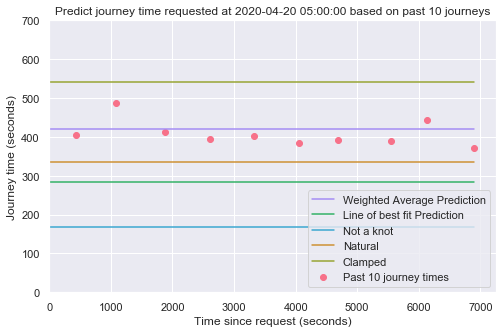
\includegraphics[keepaspectratio, width=13cm]{Images/regression-part2-comparison.png}
    \caption{Part 2 prediction comparison}
    \label{fig:part2-comparison}
\end{center}
\end{figure}

The combined regression + interpolation model that gives the final prediction result uses linear interpolation of $y_{pred1}$ from the `global' prediction and $y_{pred2}$ from the `local' prediction. The $\alpha$ parameter needs to be tuned and the resulting RMSE and MAE scores are seen in Figures \ref{fig:regression-part2weightedavg}, \ref{fig:regression-part2lineofbestfit} and \ref{fig:regression-part2cubicspline}. \\

Figure \ref{fig:regression-part2weightedavg} shows how the RMSE and MAE changes for the combined model where the part 2 model is the weighted average model. $\alpha$ was initially varied from 0 to 1, however, results showed that the dip in the MAE and RMSE occurred closer to 0, and hence the values that it was varied over was changed to between 0 and 0.2. The optimal result comes at $\alpha$ = 0.094737 (5sf), giving a MAE of 157.69 (5sf) or $\alpha$ = 0.031579 (5sf), giving a RMSE of 267.87 (5sf). A value of $\alpha$ close to 0 implies that $y_{pred1}$ is not as important as $y_{pred2}$. In other words, this result says that the predicted journey time of a bus relies mostly on the journey times of the recent buses and does not rely as much on `global' factors such as the time of day or the day of the week.

\begin{figure}[H]
\begin{center}
    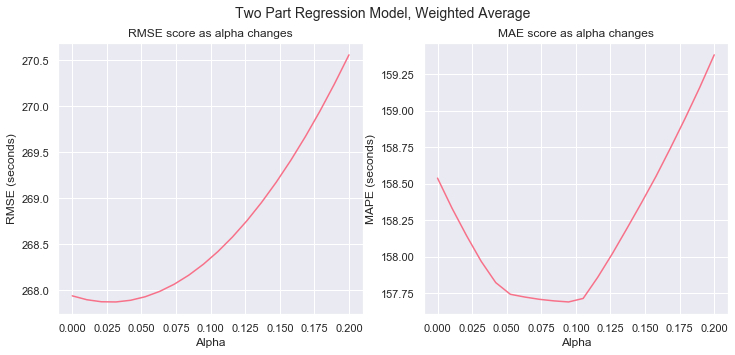
\includegraphics[keepaspectratio, width=15cm]{Images/regression-combined-weightedavg.png}
    \caption{Part 2 = Weighted Average}
    \label{fig:regression-part2weightedavg}
\end{center}
\end{figure}

Figure \ref{fig:regression-part2lineofbestfit} shows how the RMSE and MAE changes for the combined model where the part 2 model is the linear regression model. $\alpha$ was initially varied from 0 to 1, however, results showed that the dip in the MAE and RMSE occurred closer to 1, and hence the values that it was varied over was changed to between 0.8 and 1. The optimal result comes at $\alpha$ = 0.98947 (5sf), giving a MAE of 220.19 (5sf) or $\alpha$ = 0.97895 (5sf), giving a RMSE of 339.23 (5sf). A value of $\alpha$ close to 1 implies that $y_{pred2}$ is not as important as $y_{pred1}$. In other words, this result says that the predicted journey time of a bus relies mostly on `global' factors such as the time of day or the day of week, and doesn't rely as much on recent journey times.

\begin{figure}[H]
\begin{center}
    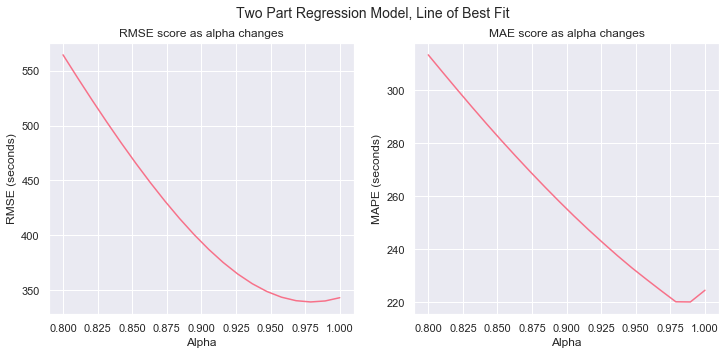
\includegraphics[keepaspectratio, width=15cm]{Images/regression-combined-lineofbestfit.png}
    \caption{Part 2 = Linear regression}
    \label{fig:regression-part2lineofbestfit}
\end{center}
\end{figure}

Figure \ref{fig:regression-part2cubicspline} shows how the RMSE and MAE changes for the combined model where the part 2 model is the three different cubic spline sub-models. $\alpha$ was varied from 0 to 1, but it can be seen that the MAE and RMSE are significantly big (note the scaale of the y axis). Therefore, cubic spline sub-models are not suitable to be used as the part 2 prediction model. Due to the nature of cubic splines and interpolations of polynomials of degree greater than two, it makes sense that they do not provide the best results. In particular, when the last 10 journeys are further away from the time of request, the intercept of the cubic spline polynomial will be at an extreme value (for example in the case where a request is made at 05:30 and the last 10 journeys are from midnight or before).

\begin{figure}[H]
\begin{center}
    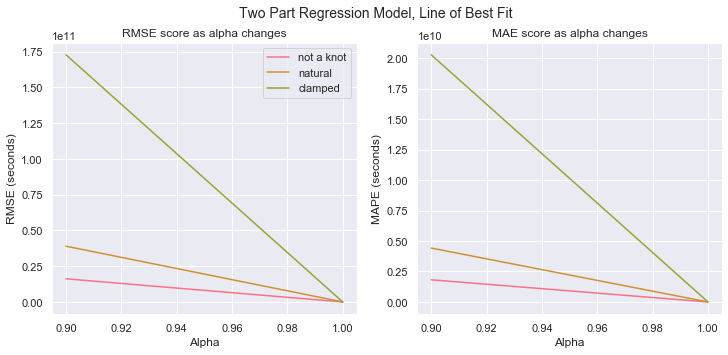
\includegraphics[keepaspectratio, width=15cm]{Images/regression-combined-cubicspline.png}
    \caption{Part 2 = Cubic Spline}
    \label{fig:regression-part2cubicspline}
\end{center}
\end{figure}

The initial hypothesis was that $\alpha$ would be in the region of 0.5. However, the results gotten have $\alpha$ at the extremes near 0 or 1. This does not support the belief that the journey time of a bus relies equally on `global' factors and `local' factors. In Figure \ref{fig:regression-comparison-allgaps} it can be seen that the combined model with the weighted average model as the part 2 model out performs linear regression as the part 2 model. In this case, the value of $\alpha$ that led to the optimal model is closer to 0, implying that bus journey prediction models should rely more on recent journey times. This supports the argument that dynamic models are more suitable than static models.

\begin{figure}[H]
\begin{center}
    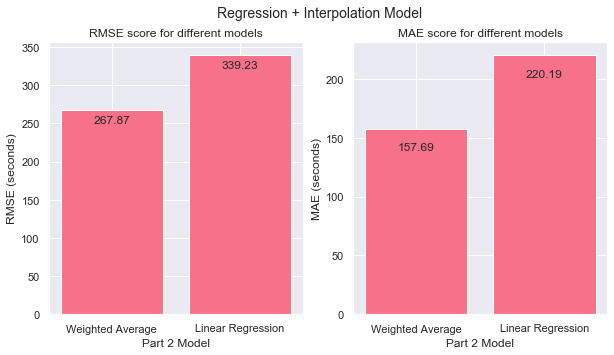
\includegraphics[keepaspectratio, width=13cm]{Images/regression-comparison-allgaps.png}
    \caption{All Gap size comparison}
    \label{fig:regression-comparison-allgaps}
\end{center}
\end{figure}

Figure \ref{fig:regression-gap5-journey-comparison} shows the prediction made by the best combined regression model (where the part 2 model is a weighted average model and $\alpha$ = 0.97895) vs TfL Countdown's predictions versus the actual journey times. This particular graph is for stops that are 5 apart, so that it is more comparable to the historical model. The figure shows that the combined model regularly under predicts the journey time.

\begin{figure}[H]
\begin{center}
    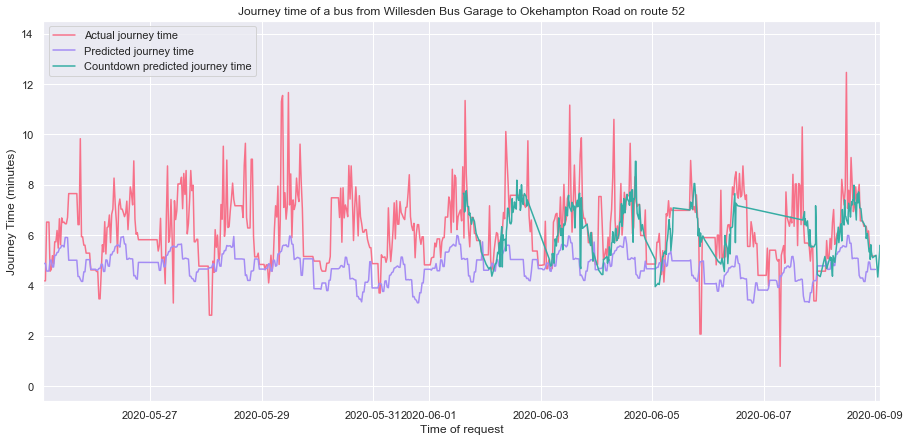
\includegraphics[keepaspectratio, width=15cm]{Images/regression-journey-comparison.png}
    \caption{Regression Model}
    \label{fig:regression-gap5-journey-comparison}
\end{center}
\end{figure}

\subsection{Cross Model Comparison}

Figure \ref{fig:all-model-comparison-gap5} shows the RMSE and MAE of all the 8 complete models compared against TfL Countdown's scores. The scores are for stops that are 5 apart. \\

By RMSE, Figure \ref{fig:all-model-comparison-gap5} shows that the best model is the combined model with the part 2 model being the weighted average model. This model also outperforms TfL Countdown's model, which is one of the aims that this project set out to do. Therefore, this can be seen as a success. However, although this model is also the best model according to MAE, it does not outperform TfL Countdown's model using this measure. Outperforming on the RMSE means that this model is less likely than the TfL model to predict values that are significantly larger or smaller than the actual value. However, under performing on the MAE means this model is not as consistent in its predictions as the TfL model. It should be noted that the difference between the scores for the two models is very small, approximately 5 seconds for both MAE and RMSE. Therefore, it could make sense to conclude that the two models are equally good. Furthermore, the range of scores achieved for stops that are five apart is not large, with the scores suggesting that all of the models are predicting within two minutes of the actual time. \\

\begin{figure}[H]
\begin{center}
    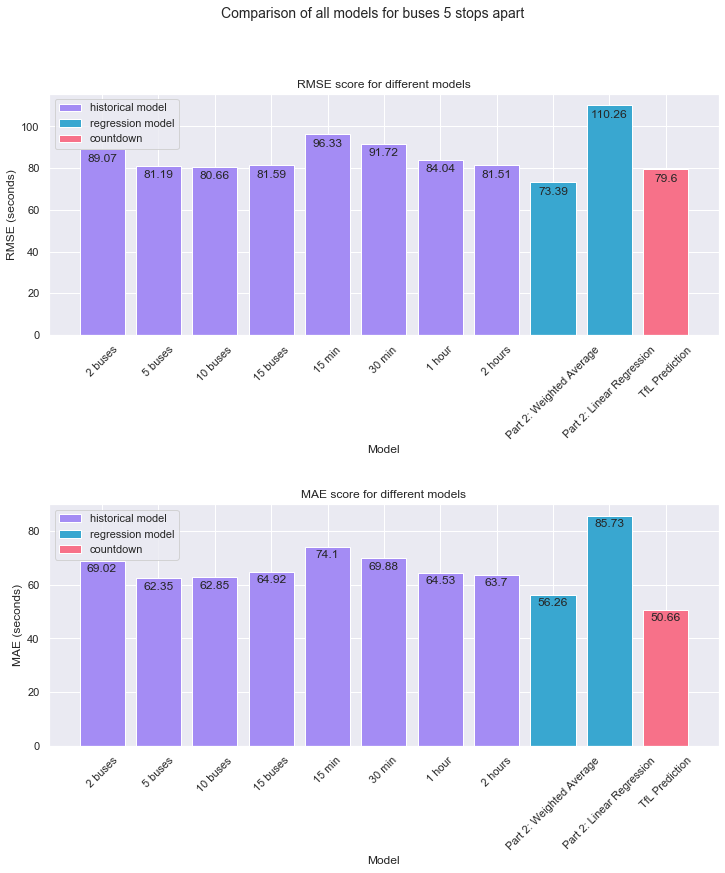
\includegraphics[keepaspectratio, width=15cm]{Images/evaluation-all-comparison-gap5.png}
    \caption{All Model Comparison Gap 5}
    \label{fig:all-model-comparison-gap5}
\end{center}
\end{figure}

Figure \ref{fig:all-model-comparison} shows the RMSE and MAE of all the top two historical models and top two regression models compared against TfL Countdown's scores. The scores are for stops of all gap sizes. \\

Unlike with looking at just stops that are five apart, Figure \ref{fig:all-model-comparison} shows that the four models presented all out perform TfL Countdown's model on both MAE and RMSE. This is a great achievement as this was one of the goals of the project - to be able to create a model that is better than TfL's own. According to the MAE, the four models developed in this project predict results that are four minutes, four minutes, two and a half minutes and three and a half minutes respectively off from the actual time. Realistically, for journeys that take longer than fifteen minutes, an extra two to four minutes does not make much of a difference. TfL's predictions on the other hand are on average about six minutes off from the actual time. Since the RMSE indicates when bigger errors are present, Figure \ref{fig:all-model-comparison} suggests that the two historical models and the combined model with the weighted average model as the part 2 model, are fairly equal in not giving outlandishly larger or small predictions. However, by the MAE it is clear that the combined model with the weighted average model as the part 2 model far exceeds the predictions made with the other models.

\begin{figure}[H]
\begin{center}
    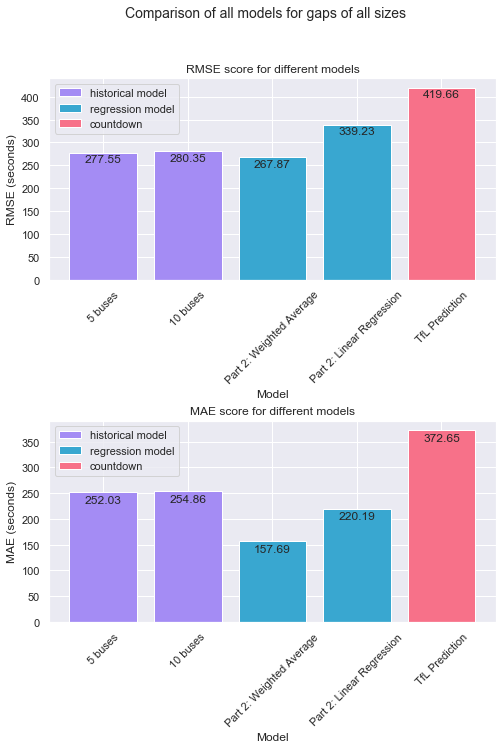
\includegraphics[keepaspectratio, width=15cm]{Images/evaluation-allmodels-allgaps.png}
    \caption{All Model Comparison}
    \label{fig:all-model-comparison}
\end{center}
\end{figure}

It is surprising that the historical models that do not take any of the `global' factors into account still perform fairly well. This could perhaps be explained by the idea that the recent journeys already take into account the `global' factors such as time of day or traffic conditions without these factors having to be explicitly found.

\clearpage